\title{Grunnatriði}
\author{Bergur Snorrason}
\date{\today}

\begin{document}

\frame{\titlepage}

\section{Grunntög}
\env{frame}
{
    \frametitle{Grunntög og takmarkanir þeirra}
    \env{itemize}
    {
        \item<1-> Í grunninn snýst forritun um gögn.
        \item<2-> Þegar við forritum flokkum við gögnin okkar með \emph{tögum}.
        \item<3-> Dæmi um tög í \ilcode{C/C++} eru \ilcode{int} og \ilcode{double}.
        \item<4-> Helstu tögin í \ilcode{C/C++} eru (yfirleitt):
        \item<5->[]
        \env{tabular}
        {
            {l l l}
            Heiti & Lýsing & Skorður\\
            \ilcode{int} & Heiltala & Á bilinu $[-2^{31}, 2^{31} - 1]$\\
            \ilcode{unsigned int} & Heiltala & Á bilinu $[0, 2^{32} - 1]$\\
            \ilcode{long long} & Heiltala & Á bilinu $[-2^{63}, 2^{63} - 1]$\\
            \ilcode{unsigned long long} & Heiltala & Á bilinu $[0, 2^{64} - 1]$\\
            \ilcode{double} & Fleytitala & Takmörkuð nákvæmni\\
            \ilcode{char} & Heiltala & Á bilinu $[-128, 127]$\\
        }
    }
}

\section{Hvað með stórar tölur?}
\env{frame}
{
    \frametitle{Hvað með tölur utan þessa bila?}
    \env{itemize}
    {
        \item<1-> Einn helsti kostur \ilcode{Python} í keppnisforritun er að heiltölur geta verið eins stórar (eða litlar) og vera skal.
        \item<2->[] \code{code/factorial.py}
        \item<3->[] \code{code/factorial.out}
        \item<4-> Það er einnig hægt að nota \ilcode{fractions} pakkann í \ilcode{Python} til að vinna með fleytitölur án þess að tapa nákvæmni.
    }
}

\section{Hvað með stórar tölur í C?}
\env{frame}
{
    \frametitle{Hvað með tölur utan þessa bila?}
    \env{itemize}
    {
        \item<1-> Sumir \ilcode{C/C++} þýðendur bjóða upp á gagnatagið \ilcode{\_\_int128} (til dæmis \ilcode{gcc}).
        \item<2-> Þetta tag býður upp á að nota tölur á bilinu $[-2^{127}, 2^{127} - 1]$.
        \item<3-> Þetta þarf ekki að nota oft.
    }
}

\section{Röðun}
\subsection{Yfirlit}
\env{frame}
{
    \frametitle{Röðun}
    \env{itemize}
    {
        \item<1-> Við munum reglulega þurfa að raða gögnum í einhverja röð.
        \item<2->[]
        \env{tabular}
        {
            {l l}
            Forritunarmál & Röðun\\
            \hline
            \ilcode{C} & \ilcode{qsort(...)}\\
            \ilcode{C++} & \ilcode{sort(...)}\\
            \ilcode{Python} & \ilcode{this.sort()} eða \ilcode{sorted(...)}\\
        }
        \item<3-> Skoðum nú hvert forritunarmál til að sjá nánar hvernig föllin eru notuð.
    }
}

\subsection{Röðun í C++}
\env{frame}
{
    \frametitle{Röðun í \ilcode{C++}}
    \env{itemize}
    {
        \item<1-> Í grunninn tekur \ilcode{sort(...)} við tveimur gildum.
        \item<2-> Fyrra gildið svarar til fyrsta staks þess sem við viljum raða og seinna gildið vísar á enda þess sem við viljum raða
            (ekki síðasta stakið)
        \item<3-> Ef við erum með $n$ staka fylki \ilcode{a} þá röðum við því með \ilcode{sort(a, a + n)}.
        \item<4-> Við getum raðað flestum ílátum með \ilcode{sort}.
        \item<5-> Ef við erum með eitthvað ílát (til dæmis \ilcode{vector}) \ilcode{a} má raða með \ilcode{sort(a.begin(), a.end())}.
        \item<6-> Við getum líka bætt við okkar eigin samanburðarfalli sem þriðja inntak.
        \item<7-> Það kemur þá í stað ,,minna eða samasem'' samanburðarins sem er sjálfgefinn.
    }
}

\subsection{Röðun í Python}
\env{frame}
{
    \frametitle{Röðun í \ilcode{Python}}
    \env{itemize}
    {
        \item<1-> Til að raða lista í \ilcode{Python} þá má nota annað hvort \ilcode{this.sort()} eða \ilcode{sorted(...)}.
        \item<2-> Gerum ráð fyrir að listinn okkar heiti \ilcode{a}.
        \item<3-> Þá nægir að kalla á \ilcode{a.sort()} og eftir það er \ilcode{a} raðað.
        \item<4-> Hinsvegar skilar \ilcode{sorted(a)} afriti af \ilcode{a} sem hefur verið raðað.
        \item<5-> Til að raða \ilcode{a} á þennan hátt þarf \ilcode{a = sorted(a)}.
        \item<6-> Nota má inntakið \ilcode{key} til að raða eftir öðrum samanburðum.
        \item<7-> Það er einnig inntak sem heitir \ilcode{reverse} sem er Boole gildi sem leyfir auðveldlega að raða öfugt.
    }
}

\subsection{Röðun í C}
\env{frame}
{
    \frametitle{Röðun í \ilcode{C}}
    \env{itemize}
    {
        \item<1-> Í \ilcode{C} er enginn sjálfgefinn samanburður, svo við þurfum alltaf að skrifa okkar eigið samanburðarfall.
        \item<2-> Til röðunar notum við fallið \ilcode{qsort(...)}.
        \item<3-> Fallið tekur fjögur viðföng:
        \env{itemize}
        {
            \item<4-> \ilcode{void *a}. Þetta er fylkið sem við viljum raða.
            \item<5-> \ilcode{size\_t n}. Þetta er fjöldi staka í fylkinu sem \ilcode{a} svarar til.
            \item<6-> \ilcode{size\_t s}. Þetta er stærð hvers staks í fylkinu okkar (í bætum).
            \item<7-> \ilcode{int (*cmp)(const void*, const void*)}. Þetta er samanburðarfallið okkar.
        }
        \item<8-> Síðasta inntakið er kannski flókið við fyrstu sýn en er einfalt fyrir okkur að nota.
        \item<9-> Þetta er \emph{fallabendir} (e. \emph{function pointer}) ef þið viljið kynna ykkur það frekar.
    }
}

\subsection{Útfærsla á röðun í C}
\env{frame}
{
    \frametitle{Röðun í \ilcode{C}}
    \selectcode{code/sort.c}{1}{27}
}

\section{Uppsetning dæma}
\env{frame}
{
    \frametitle{Uppsetning dæma}
    \env{itemize}
    {
        \item<1-> Dæmin sem við sjáum á Kattis eru (oftast) af stöðluðu sniði.
        \env{itemize}
        {
            \item<2-> Saga.
            \item<3-> Dæmið.
            \item<4-> Inntaks -og úttakslýsingar.
            \item<5-> Sýnidæmi.
        }
        \item<6-> Fyrstu tveir punktarnir geta verið blandaðir saman.
        \item<7-> Þeir eru líka lengsti hluti dæmisins.
}
}
\section{Dæmi um dæmi}
\env{frame}
{
    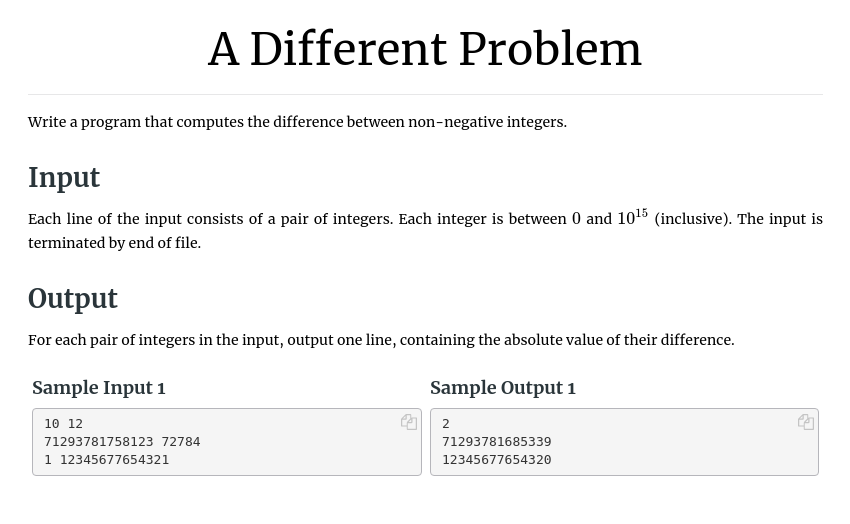
\includegraphics[scale = 0.38]{fig/daemi}
}

\section{Röng lausn}
\env{frame}
{
    \frametitle{Röng lausn. Hver er villan?}
    \code{code/differentint.cpp}
}

\section{Rétt lausn}
\env{frame}
{
    \frametitle{Rétt lausn}
    \code{code/different.cpp}
}

\section{Notkun typedef}
\env{frame}
{
    \frametitle{\ilcode{typedef}}
    \env{itemize}
    {
        \item<1-> Við getum notað \ilcode{typedef} til að spara okkur skriftir.
        \item<2-> Við bætum við \ilcode{typedef <gamla> <nýja>;} ofarlega í skrána.
        \item<3-> Venjan í keppnisforritun er að nota \ilcode{typedef long long ll;}.
        \item<4-> Við munum nota \ilcode{typedef} aftur í námskeiðinu.
    }
}

\section{Rétt lausn með typedef}
\env{frame}
{
    \frametitle{Rétt lausn með \ilcode{typedef}}
    \code{code/differentll.cpp}
}

\section{Hvernig vitum að lausn verði of hæg?}
\env{frame}
{
    \frametitle{\ilcode{Time Limit Exceeded}}
    \env{itemize}
    {
        \item<1-> Hvernig vitum að lausnin okkar sé of hæg?
        \item<2-> Ein leið er að útfæra lausnina, senda hana inn og gá hvað Kattis segir.
        \item<3-> Það myndi þó spara mikla vinnu ef við gætum svarað spurningunni án þess að útfæra.
        \item<4-> Einnig gæti leynst önnur villa í útfærslunni okkar sem gefur okkur \ilcode{Time Limit Exceeded} (\ilcode{TLE}).
        \item<5-> Til að ákvarða hvort lausn sé nógu hröð þá notum við \emph{tímaflækjur}.
        \item<6-> Sum ykkar þekkja tímaflækjur en önnur kannski ekki.
        \item<7-> Skoðum fyrst hvað tímaflækjur eru í grófum dráttum.
    }
}

\section{Tímaflækjur}
\env{frame}
{
    \frametitle{Tímaflækjur í grófum dráttum}
    \env{itemize}
    {
        \item<1-> Keyrslutími forrits er háður stærðinni á inntakinu.
        \item<2-> Tímaflækjan lýsir hvernig keyrslutími forritsins eykst þegar inntakið stækkar (í versta falli).
        \item<3-> Ef forritið er með tímaflækju $\mathcal{O}(f(n))$ þýðir það að keyrslutíminn vex eins og $f$ þegar $n$ vex.
        \item<4-> Til dæmis ef forritið hefur tímaflækju $\mathcal{O}(n)$ þá tvöfaldast keyrslutími þegar inntakið tvöfaldast.
        \item<5-> Til annars dæmis ef forritið hefur tímaflækju $\mathcal{O}(n^2)$ þá \onslide<6->{fjór}faldast keyrslutími þegar inntakið tvöfaldast.
        \item<7-> Við gerum ráð fyrir að grunnaðgerðirnar okkar taki fastann tíma, eða séu með tímaflækju $\mathcal{O}(1)$.
    }
}

\env{frame}
{
    \env{itemize}
    {
        \item<1-> Ef forritið okkar þarf að framkvæma $\mathcal{O}(f(n))$ aðgerð $m$ sinnum þá er tímaflækjan $\mathcal{O}(m \cdot f(n))$.
        \item<2-> Þetta er reglan sem við notum oftast í keppnisforritun.
        \item<3-> Hún segir okkur til dæmis að tvöföld \ilcode{for}-lykkja, þar sem hver \ilcode{for}-lykkja er $n$ löng, er
            $\mathcal{O}($\onslide<4->{$n^2$}$)$.
        \item<5-> Ef við erum með tvær einfaldar \ilcode{for}-lykkjur, báðar af lengd $n$, þá er forritið 
            $\mathcal{O}(n + n) = \mathcal{O}($\onslide<6->{$n$}$)$
        \item<7-> Einnig gildir að tímaflækja forritsins okkar takmarkast af hægasta hluta forritsins.
        \item<8-> Til dæmis er
            $\mathcal{O}(n + n + n + n + n^2) = \mathcal{O}($\onslide<9->{$n^2$}$)$.
    }
}

\env{frame}
{
    \frametitle{Stærðfræði}
    \env{itemize}
    {
        \item<1-> Við segjum að fall $g(x)$ sé í menginu $\mathcal{O}(f(x))$ ef til eru rauntölur $c$ og $x_0$ þannig að
                    \[
                        |g(x)| \leq c \cdot f(x)
                    \]
                    fyrir öll $x > x_0$.
        \item<2-> Þetta þýðir í raun að fallið $|g(x)|$ verður á endanum minna en $c \cdot f(x)$.
        \item<3-> Þessi lýsing undirstrikar betur að $f(x)$ er efra mat á $g(x)$, það er að segja $g(x)$ hagar sér ekki verr en $f(x)$.
    }
}

\section{Þekktar tímaflækjur}
\env{frame}
{
    \frametitle{Þekktar tímaflækjur}
    \env{itemize}
    {
        \item<1-> Tímaflækjur algengra aðgerða eru:
        \item<2->[]
        \footnotesize
        \env{tabular}
        {
            {p{3.0cm} | p{3.6cm} | p{2.4cm}}
            Aðgerð & Lýsing & Tímaflækja\\
            \hline
            Línulega leit & Almenn leit í fylki & $\mathcal{O}(n)$\\
            Helmingunarleit & Leit í röðuðu fylki & $\mathcal{O}(\log n)$\\
            Röðun á heiltölum & Röðun á heiltalna fylki & $\mathcal{O}(n \log n)$\\
            Strengjasamanburður & Bera saman tvo strengi af lengd $n$ & $\mathcal{O}(n)$\\
            Almenn röðun & Röðun með samanburði í $\mathcal{O}(T(m))$ tíma & $\mathcal{O}(T(m) \cdot n \log n)$\\
        }
    }
}

\section{Hundrað milljón aðgerða reglan}
\env{frame}
{
    \frametitle{$10^8$ reglan}
    \env{itemize}
    {
        \item<1-> Þegar við ræðum tímaflækjur er ,,tími'' ekki endilega rétt orðið.
        \item<2-> Við erum frekar að lýsa fjölda aðgerða sem forritið framkvæmir.
        \item<3-> Í keppnisforritun notum við \emph{$10^8$ regluna}:
        \env{itemize}
        {
            \item<4-> Tökum verstu tilfellin sem koma fyrir í inntakslýsingunni á dæminu,
                        stingum því inn í tímaflækjuna okkar
                        og deilum með $10^8$.
            \item<5-> Ef útkoman er minni en fjöldi sekúnda í tímamörkum dæmisins þá er lausnin okkar nógu hröð, annars er hún of hæg.
        }
        \item<6-> Þessa reglu mætti um orða sem: ``Við gerum ráð fyrir að forritið geti framkvæmt $10^8$ aðgerðir á sekúndu''.
        \item<7-> Reglan er gróf nálgun, en virkar mjög vel því þetta er það sem dæmahöfundar hafa í huga þegar þeir semja dæmi.
        \item<8-> Reglan gefur eftirfarandi töflu.
    }
}

\section{Mörk tímaflækjanna}
\env{frame}
{
    \env{tabular}
    {
        {l | l | l}
        Stærð $n$ & Versta tímaflækja & Dæmi\\
        \hline
        $\leq 10$ & $\mathcal{O}((n + 1)!)$ & TSP með tæmandi leit\\
        $\leq 15$ & $\mathcal{O}(n^22^n)$ & TSP með kvikri bestun\\
        $\leq 20$ & $\mathcal{O}(n2^n)$ & Kvik bestun yfir hlutmengi\\
        $\leq 100$ & $\mathcal{O}(n^4)$ & Almenn spyrðing\\
        $\leq 400$ & $\mathcal{O}(n^3)$ & Floyd-Warshall\\
        $\leq 10^4$ & $\mathcal{O}(n^2)$ & Lengsti sameiginlegi hlutstrengur\\
        $\leq 10^5$ & $\mathcal{O}(n \sqrt{n})$ & Reiknirit sem byggja á rótarþáttun\\
        $\leq 10^6$ & $\mathcal{O}(n \log n)$ & Röðun (og margt fleira)\\
        $\leq 10^8$ & $\mathcal{O}(n)$ & Línulega leit\\
        $\leq 2^{10^8}$ & $\mathcal{O}(\log n)$ & Helmingunarleit\\
        $> 2^{10^8}$ & $\mathcal{O}(1)$ & Ad hoc
    }
}

\section{Hvað má gera ef lausnin er of hæg?}
\env{frame}
{
    \frametitle{\ilcode{TLE} trikk}
    \env{itemize}
    {
        \item<1-> Stundum fær maður \ilcode{TLE} þótt maður sé viss um að lausnin sé nógu hröð.
        \item<2-> Ef forritið þarf að lesa eða skrifa mikið gæti það verið að hægja nóg á forritun til að gefa \ilcode{TLE}.
        \item<3-> Þegar við lesum af staðalinntaki eða skrifum á staðalúttak þarf forritið að tala við stýrikerfið.
        \item<4-> Slíkar að gerðir eru mjög hægar.
        \item<5-> Til að leysa þetta skrifa föll oft í \emph{biðminni} (e. \emph{buffer}) og prenta bara þegar það fyllist.
        \item<6-> Svona er þetta gert í \ilcode{C}.
    }
}

\env{frame}
{
    \frametitle{\ilcode{TLE} trikk}
    \env{itemize}
    {
        \item<1-> Í \ilcode{C++} er biðminnið tæmt þegar \ilcode{std::endl} er prentað.
        \item<2-> Til að koma í veg fyrir þetta er hægt að prenta \ilcode{\textbackslash n} í staðinn.
        \item<3-> Til dæmis \ilcode{cout << x << '\textbackslash n'}.
        \item<4-> Það borgar sig einnig að setja \ilcode{ios::sync\_with\_stdio(false)} fremst í \ilcode{main()}.
        \item<5-> Ef þið eruð í \ilcode{Java} er hægt að nota \ilcode{Kattio}.
        \item<6-> Það má finna á GitHub.
    }
}

\section{Innbyggðar gagnagrindur í C++}
\subsection{Yfirlit}
\env{frame}
{
    \frametitle{Innbyggðar gagnagrindur í \ilcode{C++}}
    \env{itemize}
    {
        \item<1-> Grunnur \ilcode{C++} býr yfir mörgum öflugum gagnagrindum.
        \item<2-> Skoðum helstu slíku gagnagrindur og tímaflækjur mikilvægust aðgerða þeirra.
        \item<3-> Við munum bara fjalla um gagnagrindurnar í grófum dráttum.
        \item<4-> Það er hægt að finna ítarlegra efni og dæmi um notkun á netinu.
    }
}

\subsection{Fylki}
\env{frame}
{
    \frametitle{Fylki}
    \env{itemize}
    {
        \item<1-> Lýkt og í mörgum öðrum forritunarmálum eru fylki í \ilcode{C++}.
        \item<2-> Fylki geyma gögn og eru af fastri stærð.
        \item<3-> Þar sem þau eru af fastri stærð má gefa þeim tileinkað, aðliggjandi svæði í minni.
        \item<4-> Þetta leyfir manni að vísa í fylkið í $\mathcal{O}(1)$.
        \item<5->[]
        \env{tabular}
        {
            {l | l}
            Aðgerð & Tímaflækja\\
            \hline
            Lesa eða skrifa ótiltekið stak & $\mathcal{O}(1)$\\
            Bæta staki aftast & $\mathcal{O}(n)$\\
            Skeyta saman tveimur & $\mathcal{O}(n)$\\
        }
    }
}

\subsection{vector}
\env{frame}
{
    \frametitle{\ilcode{vector}}
    \env{itemize}
    {
        \item<1-> Gagnagrindin \ilcode{vector} er að mestu leiti eins og fylki.
        \item<2-> Það má þó bæta stökum aftan á \ilcode{vector} í $\mathcal{O}(1)$.
        \item<3-> Margir nota bara \ilcode{vector} og aldrei fylki sem slík.
        \item<4->[]
        \env{tabular}
        {
            {l | l}
            Aðgerð & Tímaflækja\\
            \hline
            Lesa eða skrifa ótiltekið stak & $\mathcal{O}(1)$\\
            Bæta staki aftast & $\mathcal{O}(1)$\\
            Skeyta saman tveimur & $\mathcal{O}(n)$\\
        }
    }
}

\subsection{vector kóði}
\env{frame}
{
    \code{code/vector.cpp}
    \code{code/vector.out}
}

\subsection{list}
\env{frame}
{
    \frametitle{\ilcode{list}}
    \env{itemize}
    {
        \item<1-> Gagnagrindin \ilcode{list} geymir gögn líkt og fylki gera, en stökin eru ekki aðliggjandi í minni.
        \item<2-> Því er uppfletting ekki hröð.
        \item<3-> Aftur á móti er hægt að gera smávægilegar breytingar á \ilcode{list} sem er ekki hægt að gera á fylkjum.
        \item<4->[]
        \env{tabular}
        {
            {l | l}
            Aðgerð & Tímaflækja\\
            \hline
            Finna stak & $\mathcal{O}(n)$\\
            Bæta staki aftast & $\mathcal{O}(1)$\\
            Bæta staki fremst & $\mathcal{O}(1)$\\
            Bæta staki fyrir aftan tiltekið stak & $\mathcal{O}(1)$\\
            Bæta staki fyrir framan tiltekið stak & $\mathcal{O}(1)$\\
            Skeyta saman tveimur & $\mathcal{O}(1)$\\
        }
    }
}

\subsection{list kóði}
\env{frame}
{
    \code{code/list.cpp}
    \code{code/list.out}
}

\subsection{stack}
\env{frame}
{
    \frametitle{\ilcode{stack}}
    \env{itemize}
    {
        \item<1-> Gagnagrindin \ilcode{stack} geymir gögn og leyfir aðgang að síðasta staki sem var bætt við.
        \item<2->[]
        \env{tabular}
        {
            {l | l}
            Aðgerð & Tímaflækja\\
            \hline
            Bæta við staki & $\mathcal{O}(1)$\\
            Lesa nýjasta stakið & $\mathcal{O}(1)$\\
            Fjarlægja nýjasta stakið  & $\mathcal{O}(1)$\\
        }
    }
}

\subsection{stack kóði}
\env{frame}
{
    \code{code/stack.cpp}
    \code{code/stack.out}
}

\subsection{queue}
\env{frame}
{
    \frametitle{\ilcode{queue}}
    \env{itemize}
    {
        \item<1-> Gagnagrindin \ilcode{queue} geymir gögn og leyfir aðgang að fyrsta stakinu sem var bætt við.
        \item<2->[]
        \env{tabular}
        {
            {l | l}
            Aðgerð & Tímaflækja\\
            \hline
            Bæta við staki & $\mathcal{O}(1)$\\
            Lesa elsta stakið & $\mathcal{O}(1)$\\
            Fjarlægja elsta stakið  & $\mathcal{O}(1)$\\
        }
    }
}

\subsection{queue kóði}
\env{frame}
{
    \code{code/queue.cpp}
    \code{code/queue.out}
}

\subsection{set}
\env{frame}
{
    \frametitle{\ilcode{set}}
    \env{itemize}
    {
        \item<1-> Gagnagrindin \ilcode{set} geymir gögn án endurtekninga og leyfir hraða uppflettingu.
        \item<2->[]
        \env{tabular}
        {
            {l | l}
            Aðgerð & Tímaflækja\\
            \hline
            Bæta við staki & $\mathcal{O}(\log n)$\\
            Fjarlægja stak & $\mathcal{O}(\log n)$\\
            Gá hvort staki hafi verið bætt við  & $\mathcal{O}(\log n)$\\
        }
    }
}

\subsection{set kóði}
\env{frame}
{
    \code{code/set.cpp}
    \code{code/set.out}
}

\section{Þessi glæra er viljandi auð}
\env{frame}
{
}

\end{document}
